\section{Demonstration}
We build an online search engine to demonstrate our system.
\figref{fig:demosite} is a screenshot of the demo. This demo provides 
primary interface for searching news via action related queries.
The website consists of three columns to show the searching 
result, a search bar for entering query and on the right side is 
a collection of example queries. 

\begin{figure*}[th]
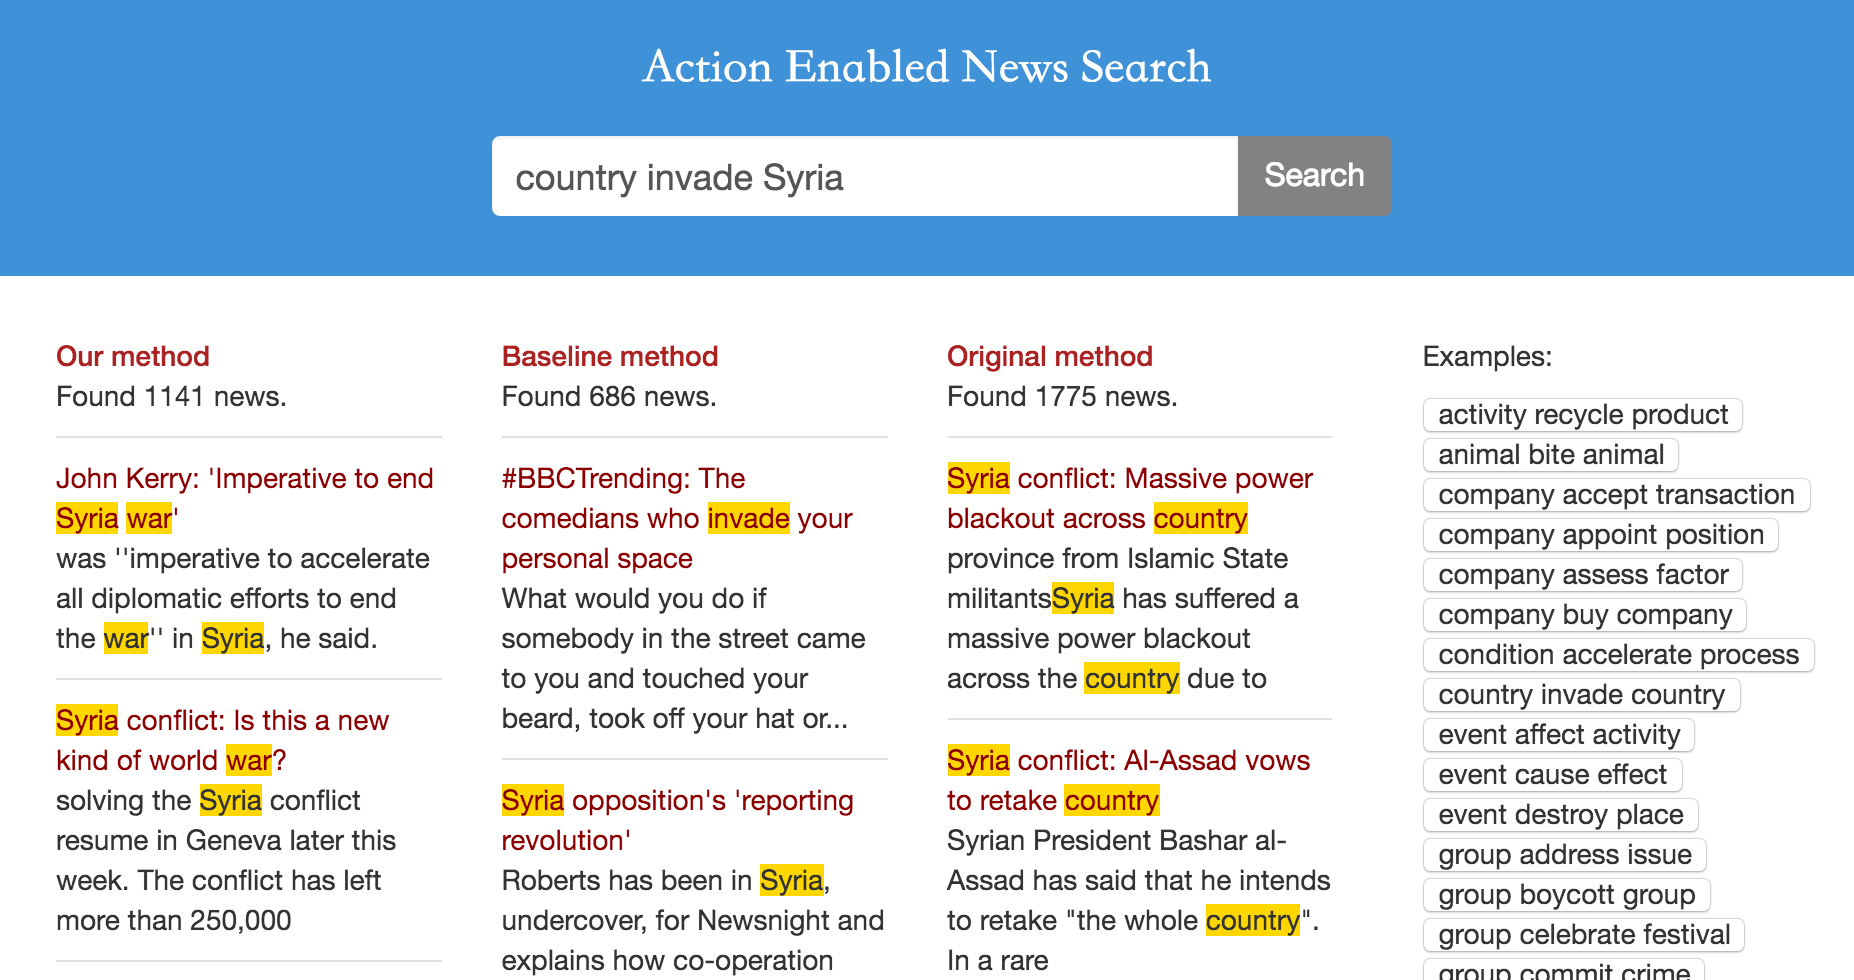
\includegraphics[width=2\columnwidth]{img/search.png}
\centering
\caption{Online demonstration}
\label{fig:demosite}
\end{figure*}


When using this demo, user can enter three types of queries. 
\begin{enumerate}
\item When input is an action concept triple, for example ``country invade country''
\item When input is an action instance triple, the query will be expanded to include the noun abstractions as well as the argument instances
\item When input is an action noun, the system can first find its action concept, then obtain the documents containing the corresponding action instances
\end{enumerate}
For case 1, we will expand the query to include the most related noun concept in the 
Action-noun mapping. So effectively ``country invade country'' will become ``invade war''.

For case 2, we first find out the argument concept of the instance,
then expand the query , but our principal is that we cannot use
general terms to query specific terms, so we need to keep the
argument instance for accuracy. So effectively ``country invade
Iraq'' will become ``invade Iraq war''.

For case 3, we need some modification of our dataset. We need to extract the action 
instances in our corpus, and consider that action instance to be one occurrence of the
noun concept as well. For example if query is ``war'' and there is a passage containing
``U.S. invaded Iraq'', then even if it might not contain ``war'' explicitly it will still be 
indexed to ``war''.

